\documentclass[10pt,a4paper]{article}
\usepackage[utf8]{inputenc}
\usepackage[T1]{fontenc}
\usepackage{amsmath}
\usepackage{amsfonts}
\usepackage{amssymb}
\usepackage{graphicx}
\usepackage{listings}
\usepackage{float}
\usepackage{multirow}
\usepackage{subcaption}
\usepackage[table]{xcolor}
\usepackage[labelformat=parens,labelsep=quad,skip=3pt]{caption}


\begin{document}
	\title{Final Exam}
	\makeatletter
	
	\author{Zackary McClamma\thanks{University of Dayton}
		\thanks{Dept. of Electrical and Computer
			Engineering, University of Dayton, 300 College Park, Dayton, OH
			45469-0226, U.S.A. E-mail:
			mcclammaz1@udayton.edu}}
	
	\makeatother
	
	\date{\today}
	
	\maketitle
	\section{Introduction}
	This project consisted of running the $\mu$C/OS-II\texttrademark operating system with three tasks. The first task blinks a green LED. The second task posts a semaphore that is unlocked by a button ISR, upon unlocking the task then increments a 7 segment display. The third task displays a user menu to a terminal with various options that are discussed in further detail in the proceeding sections of this document. Included with the submission of this document are two videos, one video is of the button, 7 segment display, and the two LEDs, the second video is a capture of the putty terminal when running the EEPROM, DMA, and SDRAM options (I found it difficult to take video with my phone that was watchable while attempting to hold it steady for 3+ minutes for the SDRAM test to complete).
	
	\section{System Design}
	This system uses i2c communications to read and write to an EEPROM device on the board. The options for telling the OS what to do are selected by a user by using the menu displayed in the terminal, the temrinal menu also includes options to run a DMA test and a SDRAM test. The system includes the Nios II processor, an I2C controller, on-chip memory (RAM), a SDRAM controller, a DMA controller, and four peripherals a red LED, a green LED, a seven segment display, and a button. The button is set up to interrupt when pressed and release a Semaphore that allows the seven segment display increment code to execute. The code for turning the green LED on and off is put in the highest priority task and it toggles the LED every 500ms (making it flash every 1 second). The rest of the pieces to this project are accessed through a terminal that runs through a COM port, the terminal will display six options Write EEPROM, Read EEPROM, Turn on Red LED, Turn off Red LED, DMA Test, and SDRAM Test. A block diagram of the system can be seen below in Figure \ref{block}

		\begin{figure}[H]
			\centering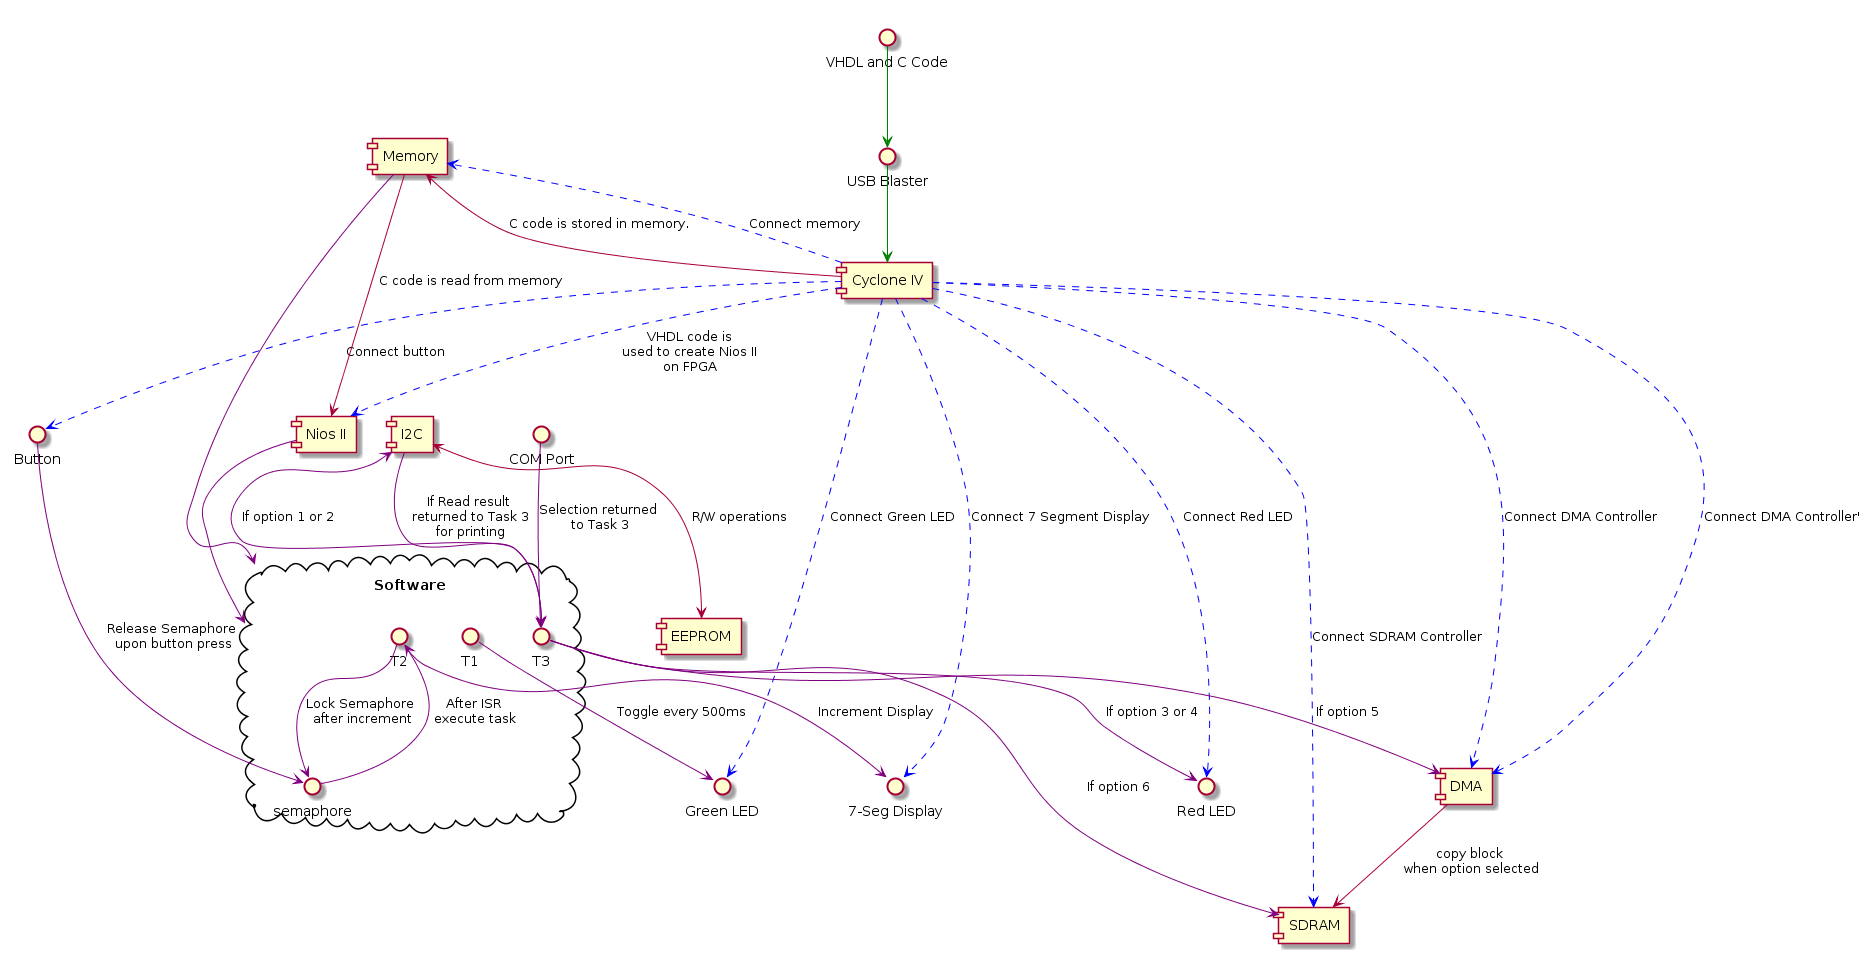
\includegraphics[width=15cm]{Final_Block_Diagram.png}
			\caption{Embedded System Block Diagram}
			\label{block}
		\end{figure}
	
	\section{Theory of Operation}
	This system runs the $\mu$C/OS-II\texttrademark operating system with three tasks. The first task toggles the green LED on and off every 500ms, this task was given the highest priority since it does not require interaction from the user and can run on its own. Making it the highest priority prevents other tasks from blocking it while waiting on input. The second task increments the seven segment display upon a button press. When the program initializes the button registers an ISR with the operating system so that when the button is pressed it triggers the button's ISR. The button ISR releases a Semaphore that is locked in the second task which calls the increment display method. The semaphore once locked waits until it is unlocked to continue executing the code below it, in this case that code is the $increment\_display()$ method. After the ISR is executed and the display is incremented the code loops back to locking the semaphore until the button ISR is triggered again.
	
	The final task in this system contains all of the menu options that are displayed in the terminal. The first and second options are Write EEPROM and Read EEPROM respectively. Write EEPROM will prompt the user for an address followed by a prompt for data, once the values are given the I2C controller will write the given data to the EEPROM at the address provided. The read EEPROM function will prompt the user for an address and the I2C controller will return the value at that address in the EEPROM. The next two options are fairly straight forward, they are Turn on Red LED and Turn off Red LED, the first will set the value of the value of the LED to 0x01 (on) and the second will set it to 0x00 (off). The final to options in the menu are DMA Test and SDRAM Test. The first will initialize a 1MB block of the SDRAM starting at the base address 0x10000000 to 0x000A0000 (NOTE: this value was arbitrarily chosen to avoid false positives that could result from using all ones or zeros, since they could just be left over from running a SDRAM test). Once the 1MB block is initialized the DMA Test then copies the 1MB block from the base address to another 1MB section starting at 0x10100000, finally it is run once more copying the block to the next 1MB chunk of memory starting at 0x10200000. The last step of each copy checks the 1MB block to ensure that the values were copied correctly. The final option on the menu is the SDRAM test, which conducts a test by writing all ones to the SDRAM, writing all zeros to the SDRAM, and writing incrementing values to the SDRAM. After each step the SDRAM is checked to ensure that the values were written properly. 
%	\begin{figure}[H]
%		\centering\includegraphics[height=15cm]}
%		\caption{Embedded System Block Diagram}
%		\label{block}
%	\end{figure}


	\section{Results}
	The EEPROM, Red LED, and the Green LED functioned normally like in the last homework assignment (the code was the base I started this project from) and the results can be seen in Figure \ref{EEPROM} below as well as in the video submitted with this document. The new additions to this project were the incrementing of the 7 segment display using a semaphore that is unlocked in the button ISR. I was able to get this to work without much issue, though I did figure out that it needed to be the second highest priority behind the blinking LED because if it was the highest it would stop the LED from blinking if the conditions are right. The SDRAM test is fairly simple write ones, then zeros, then incrementing values each time. When testing the SDRAM as you can see in Figure \ref{SDRAM} the process of writing to and reading from the SDRAM takes about 35 seconds each (meaning 35sec to read and 35sec to write), so directly writing to the SDRAM is rather slow. The DMA copy turned out to be much faster, so fast that I couldn't really get a good time estimate because the copy seemed to happen within a single clock tick, I still dont really see how this happened since I am assuming it should take multiple clock ticks to write but I guess it is only 1MB so maybe not, because of this issue where the copy was starting and finishing on the same clock tick I decided to pick a random value to write to the block so that I could ensure that my copy was actually copying something. Turns out that it was and the value was properly written to the block of SDRAM as you can see in the terminal output in Figure \ref{DMA}. 
	
	\begin{figure}[H]
		\centering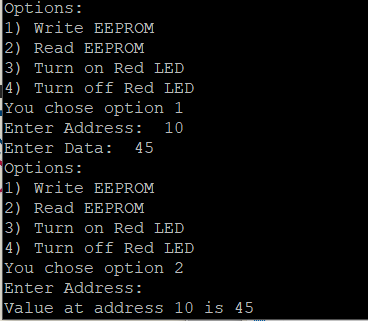
\includegraphics[height=10cm]{EEPROM_Term_Output.png}
		\caption{EEPROM Output}
		\label{EEPROM}
	\end{figure}

	\begin{figure}[H]
		\centering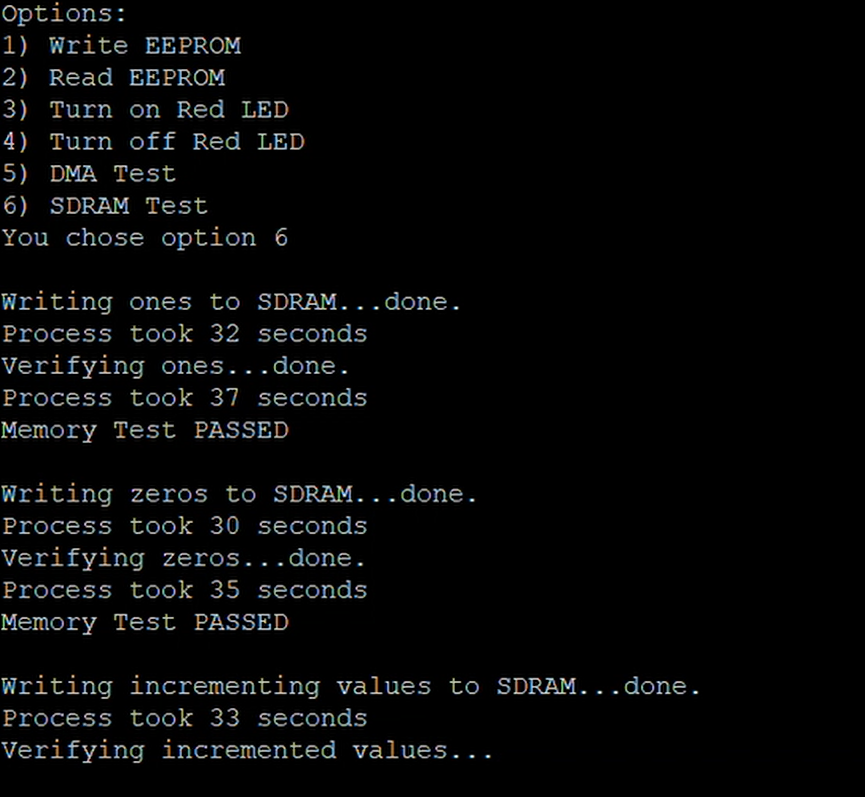
\includegraphics[height=10cm]{SDRAM_output.png}
		\caption{SDRAM Output}
		\label{SDRAM}
	\end{figure}
	\begin{figure}[H]
		\centering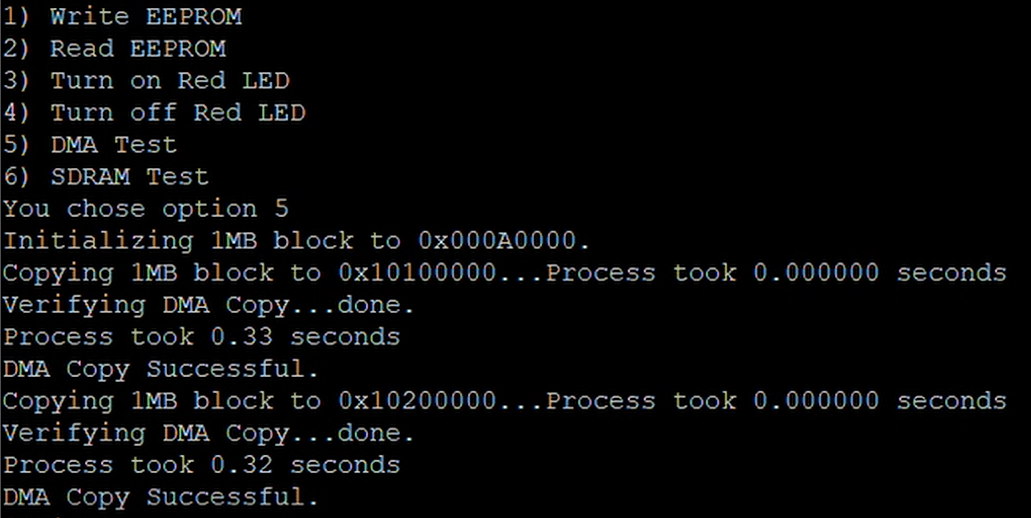
\includegraphics[height=10cm]{DMA_output.png}
		\caption{DMA Output}
		\label{DMA}
	\end{figure}
	\section{Conclusion}
	I found was able to complete the majority of this project without much trouble. The only portion that really gave me any issues was the DMA copy, I am not sure if it is just so fast that the 100MHz clock isn't fast enough to read it or what, but as I said in the results section I verified the copies each time and the data was there. I attempted to debug the timing quite a few times and every time I saw that the start and stop times I used to clock the functions were the same value every time when it came time to print them. I attempted to find a better way to clock the functions to no avail, most of the HighRes timing stuff is in C++ and this project is basically limited by the 100MHz clock when it comes to timing.
	
	\clearpage
	\appendix
	\section{\\VHDL Code}
	\lstinputlisting[language=VHDL]{final_exam.vhd}
	
	\section{\\C Code}
	\subsection{Headers}
	\lstinputlisting[language=C]{final.h}
	
	\subsection{Source}
	\lstinputlisting[language=C]{main.c}
\end{document}